\documentclass[tikz,border=2pt]{standalone}
\usepackage{amsmath,amssymb}
\usepackage{pgfplots}
\pgfplotsset{compat=1.18}

\begin{document}
% The pmf of X ~ Bin(3, 1/2): one bar per possible value, bar heights are probabilities and
% add up to 1.
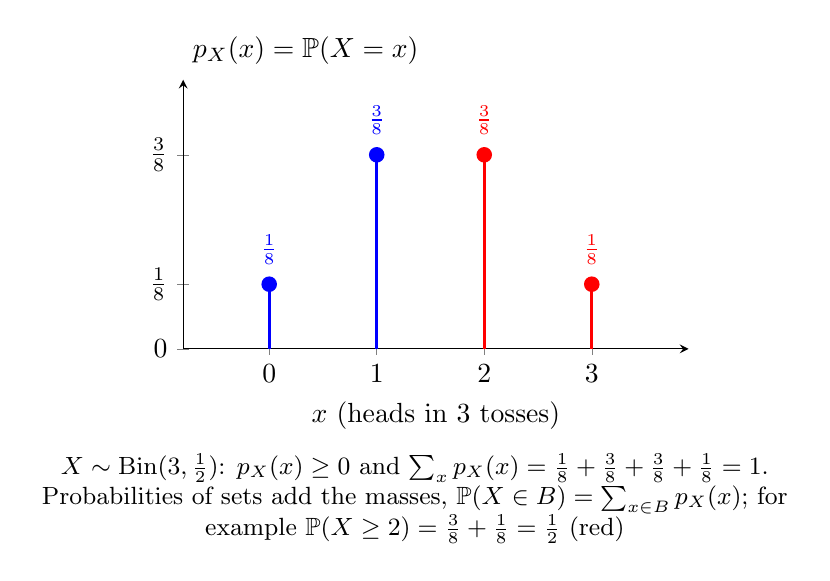
\begin{tikzpicture}
	\begin{axis}[
		axis lines=left, xmin=-0.8, xmax=3.9, ymin=0, ymax=0.52,
		xtick={0,1,2,3}, ytick={0,0.125,0.375}, yticklabels={$0$,$\tfrac18$,$\tfrac38$},
		xlabel={$x$ (heads in $3$ tosses)}, ylabel={$p_X(x)=\mathbb{P}(X=x)$}, ylabel style={rotate=-90, anchor=south west, at={(axis description cs:0,1.02)}},
		width=8cm, height=5cm, clip=false
		]
		\addplot[ycomb, blue, very thick, mark=*, mark size=2.2pt] coordinates {(0,0.125) (1,0.375)};
		\addplot[ycomb, red, very thick, mark=*, mark size=2.2pt] coordinates {(2,0.375) (3,0.125)};
		\node[blue, anchor=south, font=\small] at (axis cs:0,0.145) {$\tfrac18$};
		\node[blue, anchor=south, font=\small] at (axis cs:1,0.395) {$\tfrac38$};
		\node[red, anchor=south, font=\small] at (axis cs:2,0.395) {$\tfrac38$};
		\node[red, anchor=south, font=\small] at (axis cs:3,0.145) {$\tfrac18$};
	\end{axis}
	\node[anchor=north, font=\small, align=flush center, text width=9.6cm] at ([yshift=-2pt]current axis.outer south) {$X\sim\operatorname{Bin}(3,\tfrac12)$: $p_X(x)\ge0$ and $\sum_xp_X(x)=\tfrac18+\tfrac38+\tfrac38+\tfrac18=1$. Probabilities of sets add the masses, $\mathbb{P}(X\in B)=\sum_{x\in B}p_X(x)$; for example $\mathbb{P}(X\ge2)=\tfrac38+\tfrac18=\tfrac12$ (red)};
\end{tikzpicture}
\end{document}
